%!TEX root = informe.tex
\chapter{Análisis de Ciclo de Vida de un adoquín: interpretación}\label{cap:acv_interpretacion}

Es la fase del ACV en la que los resultados del ICV y el EICV son interpretados de acuerdo al objetivo y alcance marcados inicialmente. En esta fase se realiza un análisis de los resultados y se marcan las conclusiones.

\section{Verificación del análisis de integridad}

El objetivo de esta verificación es ``asegurar que toda la información y datos pertinentes necesarios para la interpretación están disponibles y completos'' \cite{iso14044}. La integridad asegura que no se ha olvidado ningún aspecto importante conocido.

Se ha verificado todos los procesos unitarios de todas las fases, comprobando las entradas/salidas, energía, transporte y residuos.

\section{Verificación del análisis de sensibilidad}

Hasta ahora, para calcular el perfil ambiental se ha utilizado el método ReCiPe desde la perspectiva jerárquica H. Para realizar un análisis de sensibilidad se compararán por fases los resultados con las otras perspectivas mencionadas en la sección \ref{sec:catimpactos}, la individualista (I) y la igualitaria (E).

La figura \ref{fig:sensibilidad_ia_puntuacionunica} y la tabla \ref{sensibilidad_ia_puntuacionunica} muestran los resultados usando la perspectiva individualista (I).

\begin{figure}[!htb]
\centering
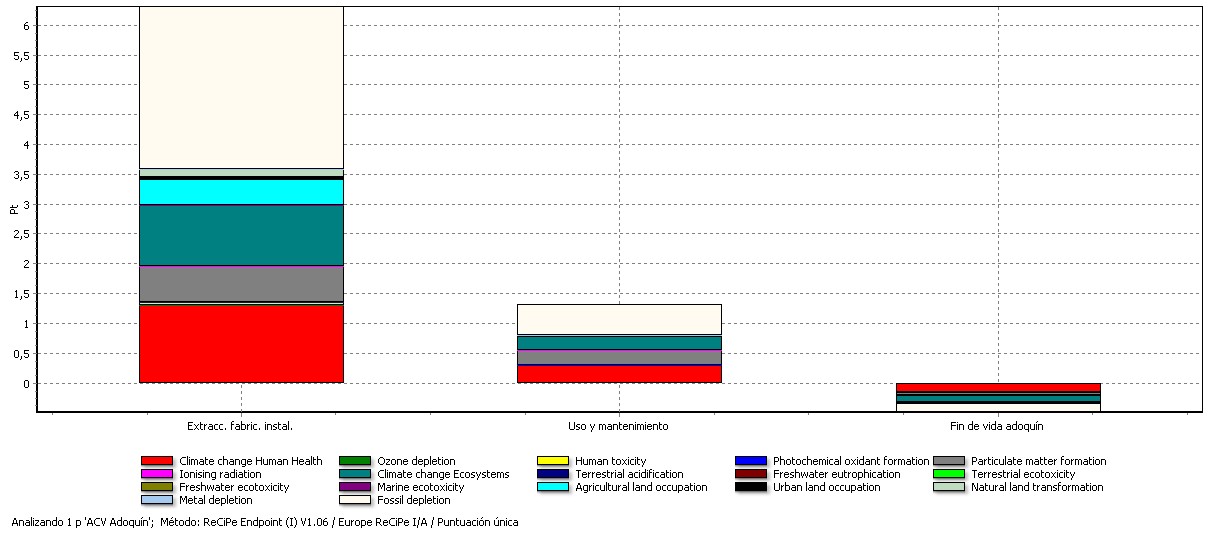
\includegraphics[width=15cm]{img/sensibilidad_ia_puntuacionunica.png}
\caption{Puntuación única por categorías de daño con el método ReCiPe I/A.}
\label{fig:sensibilidad_ia_puntuacionunica}
\end{figure}

\begin{table}[!htb]
\centering
\begin{tabular}{p{6cm}rrrr}
\toprule
\multicolumn{5}{c}{Categorías de daño puntuación única ReCiPe I/A}\\
\midrule
Etapa & Salud hum. & Ecosistema & Recursos & Total\\
 & (Pt) & (Pt) & (Pt) & (Pt)\\
\midrule
Extracc., fabric. e instal. & 1.96 & 1.61 & 2.74 & 6.31\\
Uso y mantenim. & 0.55 & 0.25 & 0.52 & 1.31\\
Fin de vida & -0.20 & -0.14 & -0.15 & -0.49\\
\bottomrule
\end{tabular}
\caption{Puntuación única por categorías de daño con el método ReCiPe I/A.}
\label{sensibilidad_ia_puntuacionunica}
\end{table}

La figura \ref{fig:sensibilidad_ia_puntuacionunica} y la tabla \ref{sensibilidad_ia_puntuacionunica} muestran los resultados usando la perspectiva individualista (I).

Por otro lado, la figura \ref{fig:sensibilidad_ea_puntuacionunica} y la tabla \ref{sensibilidad_ea_puntuacionunica} muestran los resultados usando la perspectiva igualitaria (E).

\begin{figure}[!htb]
\centering
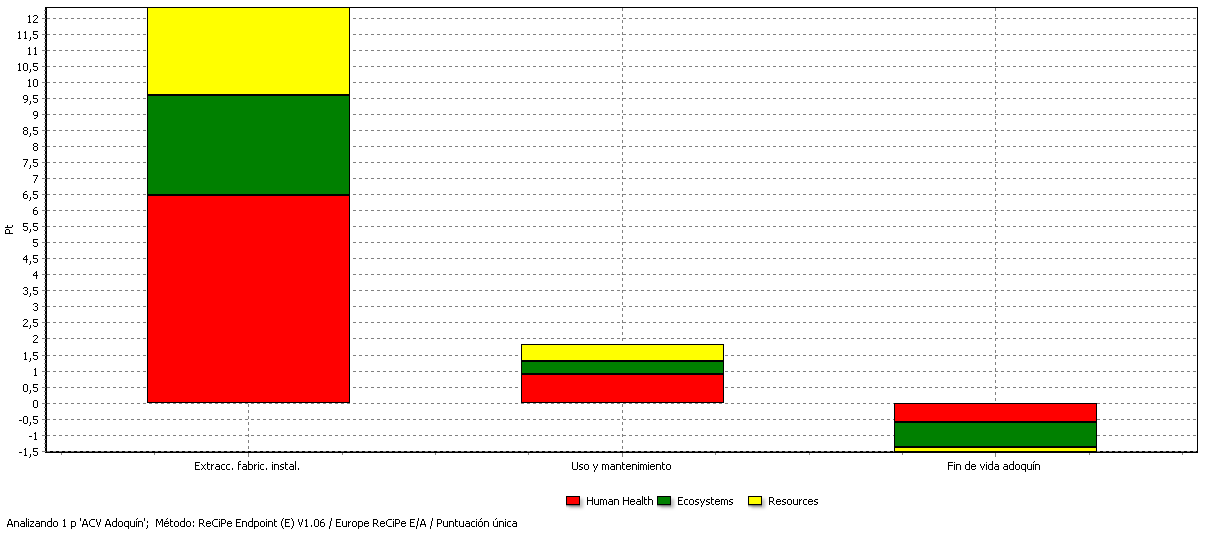
\includegraphics[width=15cm]{img/sensibilidad_ea_puntuacionunica.png}
\caption{Puntuación única por categorías de daño con el método ReCiPe E/A.}
\label{fig:sensibilidad_ea_puntuacionunica}
\end{figure}

\begin{table}[!htb]
\centering
\begin{tabular}{p{6cm}rrrr}
\toprule
\multicolumn{5}{c}{Categorías de daño puntuación única ReCiPe E/A}\\
\midrule
Etapa & Salud hum. & Ecosistema & Recursos & Total\\
 & (Pt) & (Pt) & (Pt) & (Pt)\\
\midrule
Extracc., fabric. e instal. & 6.46 & 3.13 & 2.74 & 12.3\\
Uso y mantenim. & 0.88 & 0.44 & 0.52 & 1.83\\
Fin de vida & -0.59 & -0.79 & -0.15 & -1.54\\
\bottomrule
\end{tabular}
\caption{Puntuación única por categorías de daño con el método ReCiPe E/A.}
\label{sensibilidad_ea_puntuacionunica}
\end{table}

La comparación de los resultados entre las tres perspectivas de la tabla \ref{comparativa_perspectivas} indica que las perspectivas jerárquicas e individualista tienen resultados similares, mientras que la igualitaria se diferencia bastante. Mientras que la perspectiva individualista es a corto plazo y optimista en cuanto a que la tecnología puede evitar muchos problemas en el futuro, la perspectiva igualitaria se basa a largo plazo y en una forma de pensar precavida, considerando a la naturaleza frágil e inestable, una visión fatalista poco aceptada, por lo que podría ser descartada para este proyecto, y aceptar esta parte del análisis de sensibilidad como superado.

\begin{table}[!htb]
\centering
\begin{tabular}{p{6cm}rrr}
\toprule
\multicolumn{4}{c}{Comparativa de perspectivas}\\
\midrule
Etapa & I/A & H/A & E/A\\
 & (Pt) & (Pt) & (Pt)\\
\midrule
Extracc., fabric. e instal. & 6.31 & 7.21 & 12.3\\
Uso y mantenim. & 1.31 & 1.4 & 1.83\\
Fin de vida & -0.49 & -0.543 & -1.54\\
\bottomrule
\end{tabular}
\caption{Comparativa de perspectivas H, I, E a nivel del puntuación única por categorías de daño con el método ReCiPe.}
\label{comparativa_perspectivas}
\end{table}

El análisis de sensibilidad necesita además un análisis de incertidumbre utilizando el método ReCiPe H/A con el ``Análisis Monte Carlo''. El análisis Monte Carlo es una manera numérica de procesar datos inciertos y de establecer un rango de incertidumbre en el resultado del cálculo.

\begin{figure}[!htb]
\centering
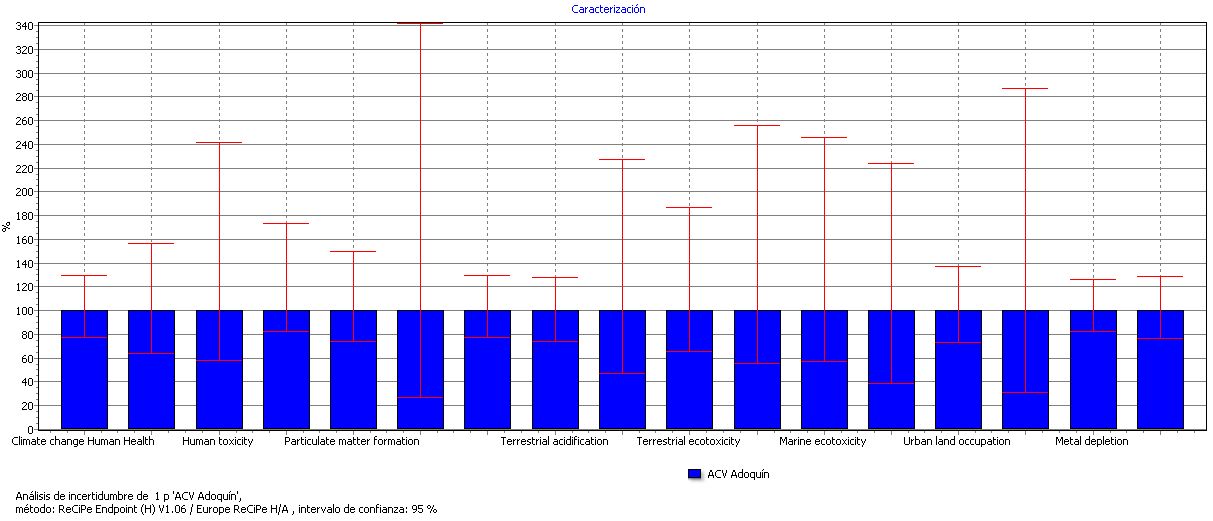
\includegraphics[width=15cm]{img/confianza_caracterizacion.png}
\caption{Intervalos de confianza para cada categoría de impacto a nivel de caracterización del ACV del adoquín.}
\label{fig:confianza_caracterizacion}
\end{figure}

Por cada categoría de impacto se indica un diagrama de barras con un margen de incertidumbre. El margen manifiesta el 95\% del intervalo de confiabilidad, lo que significa que el 95\% de los resultados estuvo dentro de este margen. Las figuras \ref{fig:confianza_caracterizacion},\ref{fig:confianza_normalizacion},\ref{fig:confianza_puntuacionunica} y \ref{fig:confianza_dano} muestran que los resultados del Análisis de Ciclo de Vida tienen una confianza del 95\%.

\begin{figure}[!htb]
\centering
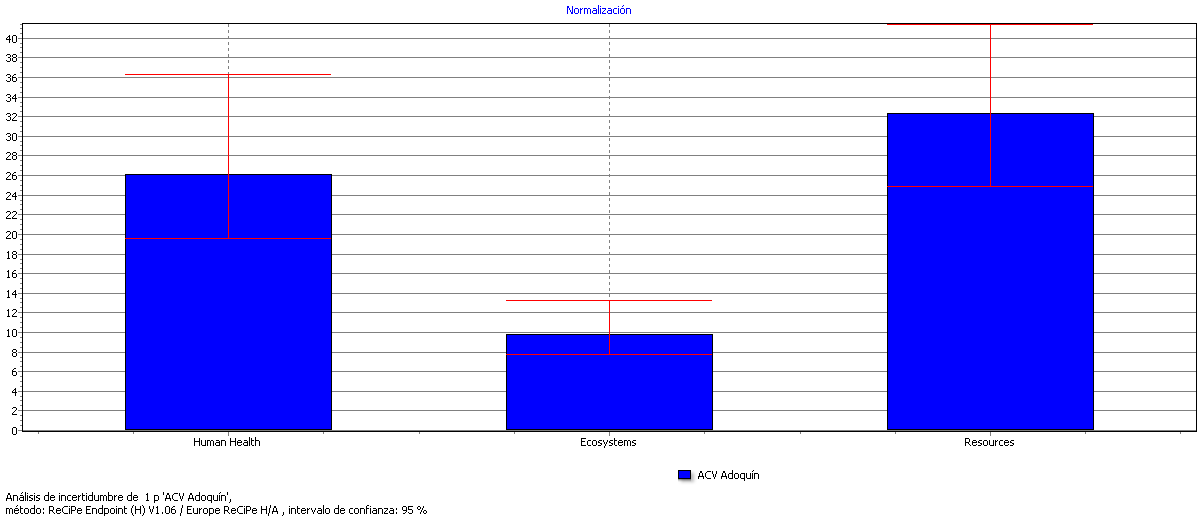
\includegraphics[width=15cm]{img/confianza_normalizacion.png}
\caption{Intervalos de confianza para cada categoría de impacto normalizada del ACV del adoquín.}
\label{fig:confianza_normalizacion}
\end{figure}

\begin{figure}[!htb]
\centering
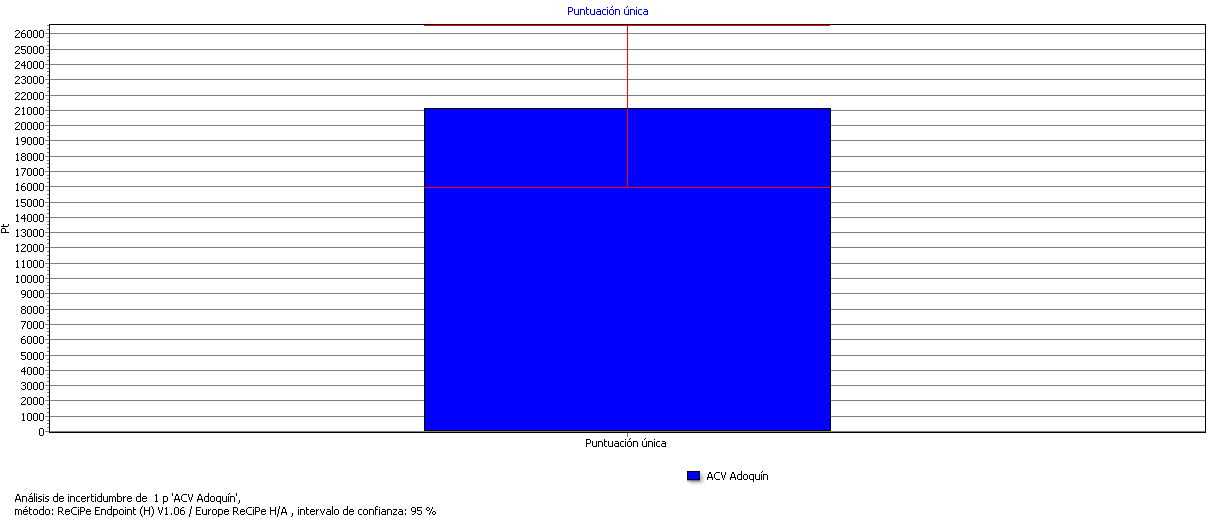
\includegraphics[width=15cm]{img/confianza_puntuacionunica.png}
\caption{Intervalos de confianza para cada categoría de impacto a nivel de puntuación única del ACV del adoquín.}
\label{fig:confianza_puntuacionunica}
\end{figure}

\begin{figure}[!htb]
\centering
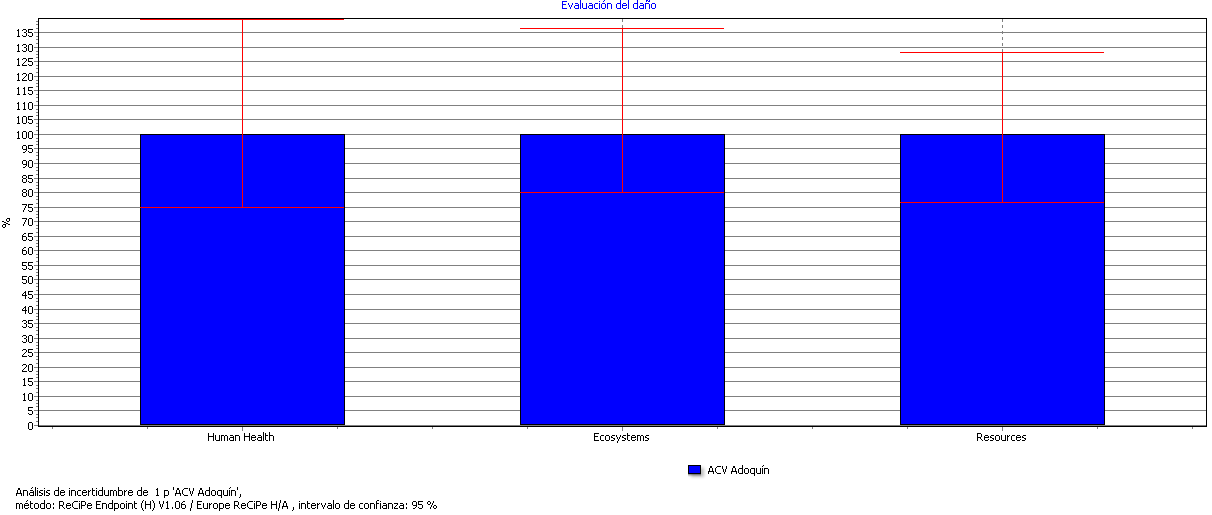
\includegraphics[width=15cm]{img/confianza_dano.png}
\caption{Intervalos de confianza para cada categoría de daño a nivel de puntuación única del ACV del adoquín.}
\label{fig:confianza_dano}
\end{figure}


\section{Verificación del análisis de coherencia}

La norma UNE-EN-ISO 14044:2006 indica que ``la verificación del análisis de coherencia busca determinar si las suposiciones, métodos, modelos y datos son coherentes a lo largo del ciclo de vida de un producto o entre distintas opciones''.

En este ACV no se realizan comparaciones entre diferentes opciones por lo que no hay comparaciones donde comprobar las incoherencias:

\begin{itemize}
  \item Fuente de datos: fabricante. Estado: OK.
  \item Exactitud de los datos: buena. Estado: OK
  \item Antigüedad de los datos: 2012—2013. Estado: OK
  \item Cobertura tecnológica: planta de fabricación. Estado: OK
  \item Cobertura relacionada con el tiempo: reciente . Estado: OK
  \item Cobertura geográfica: Málaga (España). Estado: OK
\end{itemize}

\section{Consideraciones}

El estudio del Análisis de Ciclo de Vida del adoquín indica que la etapa más influyente en el perfil medioambiental —usando el método ReCiPe—, la que mayor energía consume —con el método de Demanda de Energía Acumulada— y la que emite mayor cantidad de \ce{CO2} equivalente —por el método IPCC— es la de \textbf{extracción de materias primas, fabricación e instalación} (ver tabla \ref{perfil_medioambiental}).

\begin{table}[!htb]
\centering
\begin{tabular}{p{6cm}r}
\toprule
\multicolumn{2}{c}{Perfil medioambiental}\\
\midrule
\si{MJ} energía consumida & 1350\\
\si{kg} \ce{CO2} eq. & 58.1\\
\bottomrule
\end{tabular}
\caption{Perfil medioambiental de 1 \si{m^2} adoquín.}
\label{perfil_medioambiental}
\end{table}

\subsection{Fase de extracción de materias primas, fabricación e instalación}
Para mejorar esta fase, habrá que centrarse en los tres procesos con mayor carga ambiental que se destacaron en la tabla \ref{categoriasimpactofabricacion}.

En primer lugar, la \textbf{capa bituminosa para base granular} se compone principalmente de dos procesos:
\begin{itemize}
  \item Obtención del material bituminoso: 99.73\%.
  \item Transporte: 0.27\%.
\end{itemize}

El problema principal de los materiales bituminosos es su extracción y su refinado son altamente complejos a nivel técnico y ambiental. La extracción suele realizarse mediante minería a cielo abierto, excavando la superficie y procesando la materia prima con calor y químicos in situ para decantar el betún y permitir que este fluya a través de oleoductos. El mayor inconveniente es que el 80\% de las arenas petrolíferas se encuentran a demasiada profundidad para poder extraerlas de esta forma lo que requiere operaciones aún más complejas bajo tierra \cite{eurobitume}.

Por tanto, la única forma de poder mejorar este proceso es disminuir la distancia de transporte desde la planta de fabricación del material bituminoso hasta la zona de instalación del pavimento, lo cual no aporta una mejora cuantiosa.

En segundo lugar, el \textbf{árido grueso para base granular} se compone de dos procesos:
\begin{itemize}
  \item Obtención de la arena caliza: 67.31\%.
  \item Transporte: 32.68\%
\end{itemize}

La base granular sobre la que van el resto de capas componentes del pavimento de adoquines es la más gruesa. Sobre el proceso de obtención es difícil poder actuar ya que es proporcionada por terceros. Sin embargo, a diferencia de la capa bituminosa, sí que se puede actuar sobre la distancia de recorrido del transporte, acercando el origen donde se fabrica y la zona de instalación.

En tercer lugar, el \textbf{cemento Portland CEM I 52.5Z gris} tiene la misma problemática que los dos procesos anteriores. La distancia de transporte es muy reducida —tan sólo 8 \si{km}— y el material es proporcionado por terceros.

Por último, en referencia a todos los procesos de la etapa de extracción de materia prima, fabricación e instalación se puede actuar de forma indirecta modificando el mix eléctrico, disminuyendo la dependencia de las energías de origen fósil —que suponen un 88\% del total de la fase— y aumentando el uso de energías renovables. Debido a que las instalaciones disponen de una gran superficie, podría optarse por la instalación de paneles con células de tercera generación que permiten eficiencias de conversión eléctrica teóricas mucho mayores que las anteriores.

Desde el punto de vista ambiental, el mayor impacto se produce en las categorías de \textbf{agotamiento de recursos fósiles} y \textbf{cambio climático}, debido principalmente a los tres procesos anteriormente mencionados. La \textbf{formación de partículas} y la \textbf{ocupación de tierras agrícolas} se deben también fundamentalmente a esta fase.

\subsection{Fase de uso y mantenimiento}
Respecto a la fase de \textbf{uso y mantenimiento}, el proceso de \textbf{sellado y vibrado del pavimento} es el objetivo a mejorar. El motivo principal es el uso de combustible fósil de tipo diesel para la alimentación de la máquina de planchas vibradoras. Se puede mejorar este proceso eligiendo una máquina con el menor consumo de combustible que ofrezca el mercado.

Desde el punto de vista ambiental, el mayor impacto se produce también en las categorías de \textbf{agotamiento de recursos fósiles} y \textbf{cambio climático}, debido principalmente a sellado y vibrado del pavimento.

\subsection{Fase de fin de vida}
La etapa de \textbf{fin de vida} produce un pequeño beneficio en comparación con la primera fase, que sirve como compensación de un 61\% de la carga ambiental de la segunda fase.
